\documentclass{beamer}
\usepackage[utf8]{inputenc}
\usepackage[english,german]{babel} 
\usepackage{listings} 
\usepackage{listings-golang}

\usepackage[absolute,overlay]{textpos}
  \setlength{\TPHorizModule}{1mm}
  \setlength{\TPVertModule}{1mm}

\titlegraphic{
\includegraphics[scale=0.3]{logoHaw.png}}
\title{
	\textit{\"Ubung zur Lehrveranstaltung ``Betriebswirtschaftslehre II''} \\
	\textbf{\\ \"Ubungsblatt 1 - Gruppe 1} \\
	\scriptsize{Version 1.0}
}
\author{Adrian Helberg, \\ Thomas Bednorz \\\textbf{\\ Prüfer: Prof. Dr. M. Schultz}}
\date{\today}

\definecolor{mygreen}{rgb}{0,0.6,0}

\begin{document}
\lstset{
    frame=single,
    basicstyle=\footnotesize,
    keywordstyle=\color{blue},
    showstringspaces=false, 
    stringstyle=\color{mygreen},
    tabsize=4,
    language=Golang
}

\maketitle

\frame{\tableofcontents}

\section{Frage a) - Teil I}
\begin{frame}
\frametitle{Frage a) - Teil I}

\begin{quote}
Welche Produkte und Dienstleistungen bietet Dirt Bikes an? 
\end{quote}

\begin{itemize}
\setlength{\itemsep}{20pt}
\item Motorr\"ader vom Typ ``Offroad'', eigene Marke
\begin{itemize}
\item Verschiedene Gr\"oßen, Distanzklassen
\item Enduro 250, 550
\item Moto 300, 450
\end{itemize}
\item Ersatzteil- und Servicegesch\"aft
\item Garantiereparaturen
\end{itemize}

\end{frame}

\begin{frame}
\frametitle{Frage a)}

\begin{quote}
Wie viele Typen von Produkten und Dienstleistungen sind für die Kunden verfügbar? \\
(Konsumorientierte Betrachtung)
\end{quote}

\begin{itemize}
\setlength{\itemsep}{12pt}
\item Motorräder, Ersatzteile als
\begin{itemize}
\item Sachgut $\rightarrow$ Konsumgut $\rightarrow$ Gebrauchsgut
\end{itemize}
\item Service, Garantie als
\begin{itemize}
\item Dienstleistung $\rightarrow$ Konsumptiv $\rightarrow$ Produktbegleitend
\end{itemize}
\end{itemize}

\end{frame}

\begin{frame}
\frametitle{Frage a)}

\begin{quote}
Welches sind die wichtigsten Produkte für das Unternehmen?
\end{quote}

\begin{itemize}
\setlength{\itemsep}{20pt}
\item Hochwertige Komponenten aus der ganzen Welt (beste, verf\"ugbare Bauteile)
\begin{itemize}
\item Abheben von der Konkurrenz
\item Bekannte Markennamen als Verkaufsargument
\end{itemize}
\item Rahmen als Eigenmarke
\begin{itemize}
\item Unternehmenstypisches Aussehen $\rightarrow$ Wiedererkennungswert
\end{itemize}
\item Internes Know-how
\end{itemize}

\end{frame}

\section{Frage b)}
\begin{frame}
\frametitle{Frage b)}

\begin{quote}
Wie vertreibt das Unternehmen seine Produkte?
\end{quote}

\begin{itemize}
\setlength{\itemsep}{14pt}
\item Kein direkter Verkauf an Einzelhandelskunden
\begin{itemize}
\item Netzwerk von 40 H\"andlern
\item Unabh\"angige H\"andler f\"ur \"Ubersee (Europa)
\end{itemize}
\item Motorr\"ader, Ersatzteile und Service (einschließlich Garantiereparaturen) können nur von einem autorisierten, zertifizierten H\"andler bezogen werden
\item Bei Kunden außerhalb eines Bereichs von 50 Meilen, k\"onnen 
\begin{itemize}
\item Motorr\"ader durch einen zertifizierten, unabhängigen Motorradh\"andler gekauft werden
\item Ersatzteile direkt bei Dirt Bikes erstanden werden (Verifizierung n\"otig)
\end{itemize}
\end{itemize}

\end{frame}

\section{Frage c)}
\begin{frame}
\frametitle{Frage c)}

\begin{quote}
Welches sind die wert- und mengenm\"aßig wichtigsten Zulieferteile, die Dirt Bikes von Lieferanten bezieht?
\end{quote}

\begin{figure}
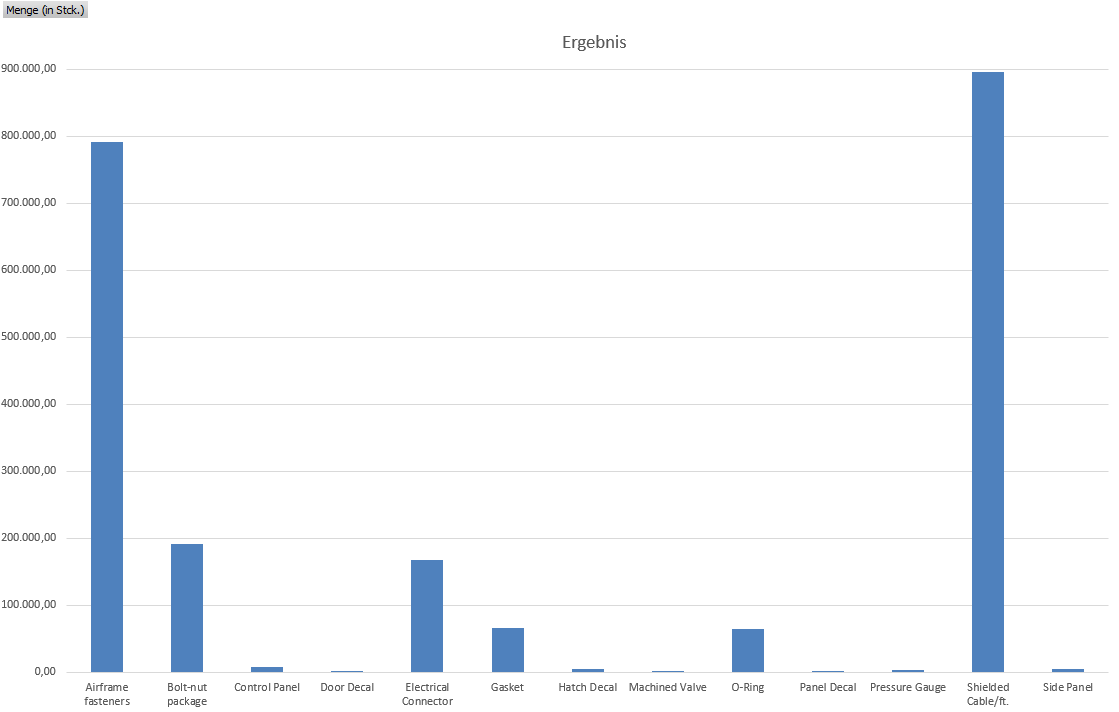
\includegraphics[scale=0.43]{pivot_itemNO_quantity.PNG}
\caption{Bestellquantit\"at pro Item Nummer (in Stck.)}
\end{figure}

\end{frame}

\begin{frame}
\frametitle{Frage c)}

\begin{quote}
Welches sind die wert- und mengenm\"aßig wichtigsten Zulieferteile, die Dirt Bikes von Lieferanten bezieht?
\end{quote}

\begin{figure}
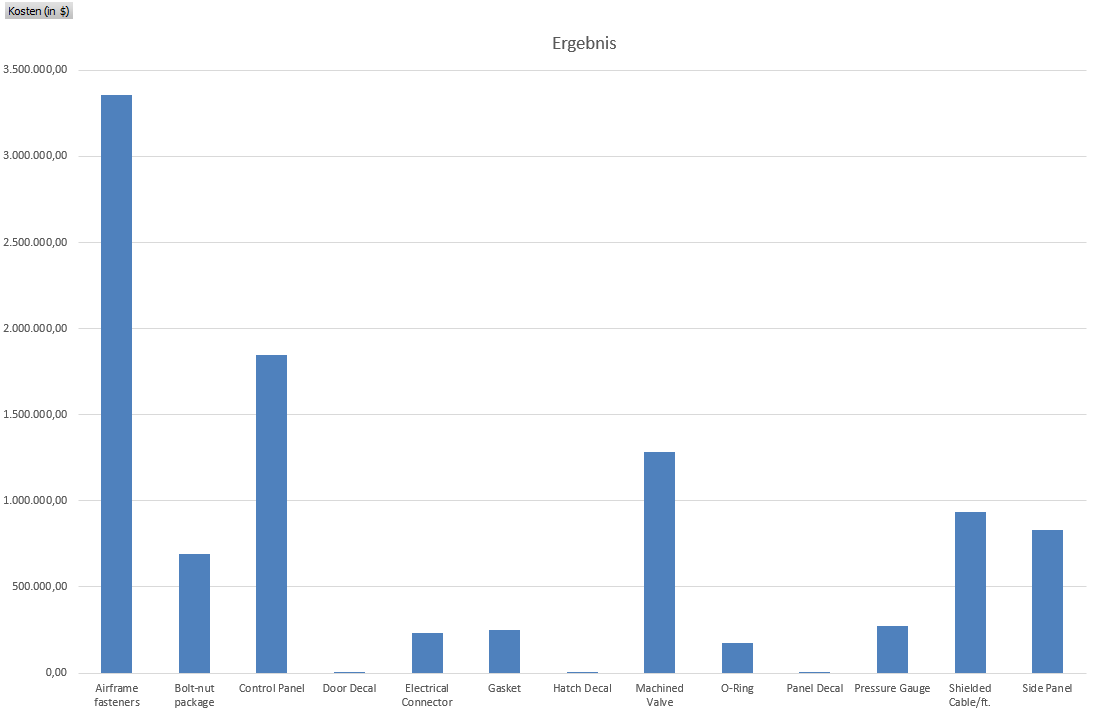
\includegraphics[scale=0.40]{pivot_itemNO_costs.PNG}
\caption{Bestellkosten pro Item Nummer (in \$)}
\end{figure}

\end{frame}

\begin{frame}
\frametitle{Frage c)}

\begin{quote}
Welches sind die wert- und mengenm\"aßig wichtigsten Zulieferteile, die Dirt Bikes von Lieferanten bezieht?
\end{quote}

\begin{itemize}
\setlength{\itemsep}{14pt}
\item Mengenm\"aßig wichtigste Zulieferteile (absteigend):
\begin{itemize}
\item Airframe fasteners (Hulkey Fasteners)
\item Shielded Cable/ft.(Fast-Tie Aerospace)
\item Shielded Cable/ft.(Steelpin Inc.)
\end{itemize}
\item Wertm\"aßig wichtigste Zulieferteile: 
\begin{itemize}
\item Airframe fasteners (Hulkey Fasteners)
\item Machined Valve (Steelpin Inc.)
\item Control Panel (Alum Sheeting)
\end{itemize}
\end{itemize}

\end{frame}

\begin{frame}
\frametitle{Frage c)}

\begin{quote}
Gibt es bei den Produkten über das Jahr auff\"allige Schwankungen?
\end{quote}

\begin{itemize}
\setlength{\itemsep}{14pt}
\item Signifikante Ausschl\"age der Kosten gibt es bei den Produktnummern 1122, 5417 und 8008 jeweils im Jannuar, Oktober und M\"arz.
Beim Produkt 1122 ist evtl. einen Großeinkauf der Ware passiert, die dann auf die folgenden Monate verteilt werden kann.
\item Signifikante Ausschl\"age der Menge gibt es bei den Produktnummern 1122, 5462  jeweils im Jannuar und Mai,
Auch hier wird evtl. die Menge auf Folgemonate verteilt.
\end{itemize}

\end{frame}

\begin{frame}
\frametitle{Frage c)}

\begin{quote}
Welches sind die wichtigsten Lieferanten für Dirt Bikes?
\end{quote}

\begin{itemize}
\setlength{\itemsep}{14pt}
\item Die wichtigsten Lieferanten sind nach Auswerten der Kosten und Mengen die Firmen ``Hulky Fasteners'' und ``Steelpin Inc.''
\end{itemize}

\end{frame}

\section{Frage d)}
\begin{frame}
\frametitle{Frage d)}

\begin{quote}
Wie ist die aktuelle Finanzielle Situation des Unternehmens (Aus Sicht des Jahres 2007)?
\end{quote}

\begin{itemize}
\setlength{\itemsep}{14pt}
\item Da keine genauen Daten zum Jahr 2007 vorliegen kann hier nur gesch\"atzt werden
\item Da sich die Summe der verkauften Motorr\"ader im Jahr 2006 auf ca. \$9292.000 bel\"auft
und im Jahre 2008 auf ca. \$9887.000, ist es wahrscheinlich, dass sich die Summe von 2007
auf ca. \$9890.000 (Mittelwert) bel\"auft
\item Die Eigenkapitalausstattung des Unternehmens ist sehr positiv
\end{itemize}

\end{frame}

\section{Frage e)}
\begin{frame}
\frametitle{Frage e)}

\begin{quote}
Welche Informationssysteme wären für ein Unternehmen wie Dirt Bikes am wichtigsten?
\end{quote}

\begin{itemize}
\setlength{\itemsep}{14pt}
\item 
\end{itemize}

\end{frame}

\begin{frame}
\frametitle{Frage e)}

\begin{quote}
Welche Schnittstellen werden zwischen den Systemen bestehen?
\end{quote}

\begin{itemize}
\setlength{\itemsep}{14pt}
\item 
\end{itemize}

\end{frame}

\section{Frage a) - Teil II}
\begin{frame}
\frametitle{Frage a) - Teil II}

\begin{quote}
Auf welche Weise k\"onnte Dirt Bikes das Internet zur Steigerung des internationalen Absatzes nutzen?
\end{quote}

\begin{itemize}
\item Das Internet k\"onnte zum elektronischen Handel (``E-Commerce'') genutzt werden
\begin{itemize}
\setlength{\itemsep}{8pt}
\item Keine Verz\"ogerung des Kaufprozesses
\item Einsicht der Produktpalette online
\item Online-Bezahlung
\item 24-Std. Service
\item Kundenn\"ahe
\item Geringe Transaktionskosten
\item Kundenkontakt auf der ganzen Welt
\end{itemize}
\end{itemize}

\end{frame}

\section{Frage b)}
\begin{frame}
\frametitle{Frage b)}

\begin{quote}
Mit welchen Merkmalen sollte die Website ausgestattet werden, um Käufer aus verschiedenen Zielländern anzuziehen?
\end{quote}

\begin{itemize}
\setlength{\itemsep}{6pt}
\item Website in englischer Sprache
\item Qualit\"at der Waren hervorheben
\item Sensible Daten sch\"utzen
\item Offenes Auftreten
\item Informationen \"uber das Unternehmen liefern
\item Verschiedene Landes-Dom\"anen  zur richtigen regionalen Ausrichtung
\item Internationale Kontaktm\"oglichkeiten
\item Uneingeschr\"ankte Verf\"ugbarkeit
\end{itemize}

\end{frame}

\end{document}